\documentclass[10pt,a4paper]{article}

\usepackage{fullpage}
\usepackage{amsmath}
\usepackage{amsfonts}
\usepackage{enumerate}
\usepackage{graphicx}

\title{Particle Filter applied to GTFS Realtime}
\author{Tom Elliott}
\date{2016}

\begin{document}

\maketitle


The Particle Filter (PF) model will allow buses to stop at bus stops
for some exponentially distributed time.
The speed component of the model will be fairly simple
(normally distributed, truncated between 0 and 30~ms$^{-1}$).
The arrival time of each particle will be recorded, 
as will the corresponding departure time. 
This should give a posterior sample of dwell times at each stop.


The condition for ``at a stop'' will be ``within 20~m of the bus stop'',
which allows for GPS error, as well as queues or other obstructions at stops.
Additionally, there will be a small probability that a bus doesn't move from its
previous location, even if its between stops (e.g., when stopped at traffic lights).



The overall state vector associated with observation $k$ is
\begin{equation}
  \label{eq:state_vector}
  X_k =
  \begin{bmatrix}
    d_k & v_k & s_k & T_{s_k} & D_{s_k}
  \end{bmatrix}^T
\end{equation}
where $d_k$ is the distance into trip (m),
$v_k$ is the speed (ms$^{-1}$),
$s_k$ is the most recently visisted stop number,
$T_j$ is the arrival time at stop $j$,
and $D_j$ the associated departure time.
The dwell time between arrival and departure at stop $j$ is $\tau_j$,
the the probability of stopping is $\pi_j$.
Each particle has its own associated state vector, denoted by a superscript $(i)$,
for example $X_k^{(i)}$.

The data are GPS coordinates and timestamps.
The elapsed time between observations is denoted $\delta_k = t_k - t_{k-1}$.
To compute likelihoods for the particles, and therefore perform weighted resampling,
the distances $d_k$ are transformed into GPS coordinates, using the shape associated
with the trip and interpolating.
The distance is thence just a great circle distance\footnote{In fact, 
the flat Earth approximation was within $1\times 10^{-15}$~m in the shape files used, 
so it will suffice if computation times need reducing. Currently, it's not an issue.}
between two points,
\begin{equation}
  \label{eq:greatcircle}
  \Delta d = R \arcsin(\sin(\phi_1) \cdot \sin(\phi_2) +
  \cos(\phi_1) \cdot \cos(\phi_2) \cdot \cos(|\lambda_1 - \lambda_2|))
\end{equation}
where $R$ is the Earth's radius is the desired units (we use $R = 6.371\times 10^6$~m).
The particle weights are based on the distances being normally distributed
with mean 0 and varince a model parameter to tune (although it is effectively GPS error).
Too small and too few particles will be resamples; too large and the accuracy will be low.


\section{Model}

There are several parts to the model:

\begin{enumerate}
\item checking step
\item movement step
\item arrival/dwell step
\item weight and update
\end{enumerate}


\subsection{Checking Step}

This requires checking of the bus' status, for example the trip ID, whether or not it has started the trip
(this can be based on time or location of the bus), or if it has finished.
Knowing about blocks would make this much easier \ldots


\subsection{Movement Step 1.0}
\label{sec:move}

Particles all drive off for $\delta_k$~seconds and see where they end up.
The speed is randomly sampled for each particle before doing so, otherwise resampled points will have the same speed,
and variation will be lost.
So, it's a two-stage step:
\begin{align*}
  v_k^{(i)} &= v_{i-1}^{(i)} + \epsilon_{k}^{(i)},\qquad \epsilon_k \sim \mathcal{N}(0, \sigma_v^2) \\
  d_k^{(i)} &=
              \begin{cases}
                d_{k-1}^{(i)} + v_k^{(i)} \delta_k, & \text{ if bus is not at a stop } \\
                d_{k-1}^{(i)} + v_k^{(i)} \left(\delta_k - \xi_k^{(i)}\right),
                &\text{ if bus is at a stop, } \quad \xi_k \sim \mathcal{E}(\tau_{s_k}^{-1})
              \end{cases}
\end{align*}
An extra condition is that $v_k^{(i)} \geq 0$ (i.e., the buses don't go backwards along the route, in theory).
Also put upper bound of 30~ms$^{-1}$ which is a little over 100~kmh$^{-1}$.


\subsection{Arrival/Dwell Step 1.0}
\label{sec:arr-dwell}

\emph{To simplify notation, for any stop-related variable $Z$, 
let the value for the $i^\mathrm{th}$ particle at time $k$ at stop $s_j = s_k^{(i)}$ 
be simply denoted $Z_j^{(i)}$, and $\omega_j$ be the underlying parameter for a given stop $j$.}

\bigskip\noindent
At some point, the bus will drive past and possibly (probably?) stop at (or near) a bus stop.
The probability of this happening is $\pi_j$, so $p_j^{(i)} \sim \mathrm{Bern}(\pi_j)$ 
indicates whether or not each particle stops.
Regardless of whether the bus stops or not, the arrival time is
\begin{equation}
  \label{eq:arrival_time}
  T_j^{(i)} = d_{k-1}^{(i)} + \frac{s_j - d_{k-1}^{(i)}}{v_k^{(i)}}
\end{equation}

If the bus doesn't stop (i.e., $p_j^{(i)} = 0$), then the departure time is the arrival time,
i.e., $D_j^{(i)} = T_j^{(i)}$.
If the bus does stop, then it stays there for $\gamma + \tau_j^{(i)}$~seconds,
where $\gamma$ is another model parameter which specifies the time taken to decelerate, open and close doors,
and accelerate again, and $\tau_j$ is the time taken for passengers to board and disembark.
From here, either
\begin{enumerate}[i.]
\item 
  $T_j^{(i)} + \gamma + \tau_j^{(i)} \geq t_k$, in which case the bus remains at the bus stop, 
  and $d_k^{(i)} = d_j^{(i)}$ (the distance into trip of the stop), or
\item 
  $T_j^{(i)} + \gamma + \tau_j^{(i)} < t_k$, in which case the bus departs the stop and carries on.
  In this case, the departure time is set to
  \begin{equation}
    \label{eq:departure_time}
    D_j^{(i)} = T_j^{(i)} + \gamma + \tau_j^{(i)},
  \end{equation}
  and the remaining travel time is $t_k - D_j^{(i)}$, so the new distance is computed to be
  \begin{equation}
    \label{eq:distance_after_stopping}
    d_k^{(i)} = d_{s_k}^{(i)} + v_k^{(i)} \left( t_k - D_j^{(i)} \right).
  \end{equation}
  In this case, it is necessary to repeat the arrival/dwell step in case the bus makes it to other stops
  (for example, if a bus fails to report for an extra long time period, or if there are several stops
  close together).
\end{enumerate}


\subsection{Weight and Update Step 1.0}
\label{sec:weight-update}

Once the particles have been moved forward and their locations finalised, the data point is used to 
obtain the likelihood weights of them.
First, the particle distances $d_k$ are transformed into GPS coordinates using the trip's associated 
shape file. 
That is, $r_k^{(i)} = h(d_k^{(i)})$, where $r_k = [\phi_k, \lambda_k]^T$, the longitude and latitude
respectively.
The distance between points is computed using (\ref{eq:greatcircle}), 
and the weights of each particles are
\begin{equation}
  \label{eq:particle_weights}
  w^{(i)} = \frac{p(Y_k | X_k^{(i)})}{\sum_{j=1}^M p(Y_k | X_k^{(j)})}
\end{equation}
where
\begin{equation}
  \label{eq:particle_lhood}
  Y_k | X_k^{(i)} \sim \mathcal{N}\left(X_k^{(i)}, \sigma_y^2\right) \equiv
  X_k^{(i)} \sim \mathcal{N}\left(0, \sigma_y^2\right)
\end{equation}
since the data have been transformed so $Y_k = 0$.
$\sigma_y^2$ is the GPS error

The particles are then resampled based on their weights, and the resulting set is considered
a sample from the posterior distribution, from which new predictions are made once the next 
observation comes in.



\section{Issues}

Several issues with the model, caused by the way the data is collected \ldots


\subsection{Dwell time at non-stops}

Main example: traffic lights! 
Need some extra probability $\kappa_k$ that is small but probable, 
which allows particles to remain where they were at the previous observation
for some time $\eta_k \sim \mathcal{E}(\tau_b^{-1})$.
This is implemented, and the logic is exactly the same as in \S~\ref{sec:move},
but using $\eta_k$ instead of $\xi_k$.


\subsection{$\delta_k$ depends on bus speed?}

No in depth study performed yet, but it looks like buses report their position less 
frequently when they are stuck in traffic (or not moving very quickly for some other
reason).
This will influence how we model $\omega_k$ and $\kappa_k$\ldots




\begin{figure}[hb!]
  \centering
  \includegraphics[width=0.8\textwidth]{../../figs/pf_singlebus/v3787/distance_time.jpg}
  \caption{Distance into trip (km) of vehicle over course of the day.}
  \label{fig:distance-time}
\end{figure}

\begin{figure}[tbp]
  \centering
  \includegraphics[width=0.49\textwidth]{../../figs/pf_singlebus/v3787/delta_distance_time.jpg}
  \caption{Change in distance versus change in time after removing all observations where $\Delta_d \leq 0$.}
  \label{fig:delta-distance-time}
\end{figure}


Need to investigate what happens if $\kappa_k = f(\delta_k)$,
and also penalise $v_k$ using $\delta_k$ too: if $\delta_k$ is small, 
then the bus may have sped up; if it is large, the bus may have slowed down.

And of course, this is completely observational right now \ldots see Figure~\ref{fig:distance-time}
at about 8~a.m.; the gap corresponds to the right-most point in Figure~\ref{fig:delta-distance-time}.


\textbf{Update:}
This might be less common than first assumed.
Perhaps the 12~minute observation was because the driver turned the bus off? 
Or the location caused interference so the bus couldn't connect to the central server \ldots

\begin{figure}[hbt!]
  \centering
  \includegraphics[width=0.49\textwidth]{../../figs/pf_singlebus/v2933/delta_distance_time.jpg}
  \includegraphics[width=0.49\textwidth]{../../figs/pf_singlebus/v3704/delta_distance_time.jpg}
  \caption{Change in distance versus change in time for two other vehicles.}
  \label{fig:delta-distance-time2}
\end{figure}


\subsection{Particles all too far from observed location}

When computing distances in the Weight and Update Step (\S~\ref{sec:weight-update}),
it's possible that all of the particles are too far away (e.g., $>20$~m) from the 
reported position of the bus. In this situation, the likelihood of all particles
can be 0, so the weights are undefined. 
Increasing $\sigma_y^2$ would fix this, but it would mean that the particles are not 
good representations of the true position of the bus.



There are three situations when this occurs:
\begin{enumerate}[(i)]
\item 
  The true position of the bus is \emph{behind} all of the particles, due to longer dwell times
  or higher congestion than expected.

  \textbf{Detect:} if the particles nearest the reported bus position have the \emph{smallest}
  value of $d_k^{(i)}$.

  \textbf{Solution:} repeat the prediction step, increasing stopping probabilities and dwell times
  (especially if bus was previous at a stop),
  and allowing slower speeds to be sampled (in the case of heavy congestion).

\item 
  The true position of the bus is \emph{ahead of} all of the particles, due to lower than expected dwell
  times, or stopping at stops, or a break in the traffic resulting in increased speed (for example the
  appearance of a bus lane, or passing the site of an accident).

  \textbf{Detect:} if the particles nearest the reported bus position have the \emph{largest}
  value of $d_k^{(i)}$.

  \textbf{Solution:} Repeat step, reducing stopping probabilities and dwell times (for example nobody gets on or off 
  the bus for whatever reason), 
  and allowing higher speeds to be sampled (such as when passing an accident).

\item 
  The sparsity of the particles isn't even enough, so the actual observation is between particles, but they 
  are all too far away.

  \textbf{Detect:} neither (i) nor (ii) occur.

  \textbf{Solution:} rerun the simulation the same as before. If this doesn't solve the issue, it might be necessary
  to increase the number of particles for the step.
\end{enumerate}

A related issue is variance of particles weights: if only a few particles have high weights, it means that 
the model hasn't predicted too well---this can result in (iii) above. 
In this case, it is necessary to increase the number of particles.
Alternatively, if all of the particles have similar weights, there is not enough variation between them,
so the error needs to be increased.


\subsection{Backtracking Buses}

The model explicitely requires buses to move forward along the route. 
i.e., $d_k \geq d_{k-1}$.
However, it appears that GPS error can make it appear that buses travel \emph{backwards} slightly.

\textbf{Temporary fix:} increase $\sigma_y^2$ if it appears that the bus has travelled backwards, 
for just a single iteration.

\textbf{Future fix:} do an analysis of GPS error to get a better esimate of $\sigma_y^2$.
This will probably involve looking for buses stopped at a particular bus stop, 
and finding the variance of their GPS positions.
For this to work, we need to find a stop with low-frequency so the buses are stopped in $\approx$ the same position.



\subsection{End-route behaviour}

At end of route, all particles seem to end up at stops, never between them where the bus is.
Need to look at what's happening to speed/arrival/departure times.




\section{Particle Motion Prediction}
\label{sec:particle-prediction}

Predicting the future location of particles is a key step in the PF. 
It is separate from the main goal of predicting future arrival time 
(which could be 5--30~minutes into the future, or longer)
but it will provide a good ground work for that.
i.e., we can't predict 30~minutes ahead if we can't predict 30~seconds.

There are several ways we intend to attempt prediction:
\begin{itemize}
\item \textbf{dynamics}: this is what we used previously
\item \textbf{(shifted) schedule}: this uses the schedule to estimate the distance that will be traveled
\item \textbf{historical}: similar to schedule, but uses historical data instead
\item \textbf{dynamics + historical (+ schedule)}: uses a combination of these, and schedule as a fallback
\end{itemize}


\subsection{Schedule}

Ideally, this will be a baseline for prediction: before we have any historical data,
or any previous state estimates, the best guess at where the bus will be will come from
the schedule (i.e., the static arrival times at stops along the route).

It involves taking the previous distance into trip, $d_{k-1}$, 
mapping that to the scheduled \emph{time} at that distance,
then adding $\delta_k$ and obtaining the new distance, $d_k$.







\section{Arrival Time Prediction}
\label{sec:arrival_time}

Many ways to do this.
First is to just let the particles continue in their current state until they reach the stop,
including any dwell times along the way.
First, let $S_j$ be the distance into the trip of stop $j$, then the arrival time at stop $j$ is
\begin{equation}
  \label{eq:state_pred}
  T_j^{(i)} = T_0 + \frac{S_j - d_k^{(i)}}{v_k^{(i)}} + \sum_{\ell = s_k^{(i)} + 1}^{s_j} p_\ell^{(i)} (\gamma + \tau_\ell^{(i)})
\end{equation}
where $T_0$ is the departure time of the current stop if the bus hasn't left yet,
otherwise the current time.
Alternatively, $T_0$ can be 0 (or the time until departure) in which case $T_j$ will be 
the remaining time until arrival.


The second method involves using the schedule deviation.
That is, take the deviatino between actual arrival and scheduled arrival at the most recent stop,
and add that to the scheduled arrival time at the future stop(s), $\bar S_j$.
\begin{equation}
  \label{eq:sched_pred}
  T_j^{(i)} = \bar S_j + \underbrace{T_{s_k}^{(i)} - \bar S_{s_k^{(i)}}}_{\text{schedule deviation}}
\end{equation}






\end{document}
